\documentclass{article}

\usepackage{fancyhdr}
\usepackage{extramarks}
\usepackage{amsmath}
\usepackage{amsthm}
\usepackage{amsfonts}
\usepackage{tikz}
\usepackage[plain]{algorithm}
\usepackage{algpseudocode}
\usepackage{graphicx}
\usepackage{gensymb}
\usepackage[framed,numbered,autolinebreaks,useliterate]{mcode}

\graphicspath{{./images/}}

\usetikzlibrary{automata,positioning}

%
% Basic Document Settings
%

\topmargin=-0.45in
\evensidemargin=0in
\oddsidemargin=0in
\textwidth=6.5in
\textheight=9.0in
\headsep=0.25in

\linespread{1.1}

\pagestyle{fancy}
\lhead{\hmwkAuthorName}
\chead{\hmwkClass\ \hmwkTitle}
\rhead{\firstxmark}
\lfoot{\lastxmark}
\cfoot{\thepage}

\renewcommand\headrulewidth{0.4pt}
\renewcommand\footrulewidth{0.4pt}

\setlength\parindent{0pt}

%
% Create Problem Sections
%

\newcommand{\enterProblemHeader}[1]{
    \nobreak\extramarks{}{Problem {#1} continued on next page\ldots}\nobreak{}
    \nobreak\extramarks{Problem {#1} (continued)}{Problem {#1} continued on next page\ldots}\nobreak{}
}

\newcommand{\exitProblemHeader}[1]{
    \nobreak\extramarks{Problem {#1} (continued)}{Problem {#1} continued on next page\ldots}\nobreak{}
    % \stepcounter{#1}
    \nobreak\extramarks{Problem {#1}}{}\nobreak{}
}

\setcounter{secnumdepth}{0}
\newcounter{partCounter}

\newcommand{\problemNumber}{0.0}

\newenvironment{homeworkProblem}[1][-1]{
    \renewcommand{\problemNumber}{{#1}}
    \section{Problem \problemNumber}
    \setcounter{partCounter}{1}
    \enterProblemHeader{\problemNumber}
}{
    \exitProblemHeader{\problemNumber}
}

%
% Homework Details
%   - Title
%   - Class
%   - Author
%

\newcommand{\hmwkTitle}{Homework\ \#2}
\newcommand{\hmwkClass}{RBE 500}
\newcommand{\hmwkAuthorName}{\textbf{Arjan Gupta}}

%
% Title Page
%

\title{
    \vspace{2in}
    \textmd{\textbf{\hmwkClass\ \hmwkTitle}}\\
    \vspace{3in}
}

\author{\hmwkAuthorName}
\date{}

\renewcommand{\part}[1]{\textbf{\large Part \Alph{partCounter}}\stepcounter{partCounter}\\}

%
% Various Helper Commands
%

% Useful for algorithms
\newcommand{\alg}[1]{\textsc{\bfseries \footnotesize #1}}

% For derivatives
\newcommand{\deriv}[1]{\frac{\mathrm{d}}{\mathrm{d}x} (#1)}

% For partial derivatives
\newcommand{\pderiv}[2]{\frac{\partial}{\partial #1} (#2)}

% Integral dx
\newcommand{\dx}{\mathrm{d}x}

% Alias for the Solution section header
\newcommand{\solution}{\textbf{\large Solution}}

% Probability commands: Expectation, Variance, Covariance, Bias
\newcommand{\E}{\mathrm{E}}
\newcommand{\Var}{\mathrm{Var}}
\newcommand{\Cov}{\mathrm{Cov}}
\newcommand{\Bias}{\mathrm{Bias}}

\begin{document}

\maketitle

\nobreak\extramarks{Problem 3.5}{}\nobreak{}

\pagebreak

\begin{homeworkProblem}[3.5]
    Consider the three-link articulated robot of Figure 3.16. Derive the forward kinematic equations using the DH convention.
    \begin{figure}[h]
        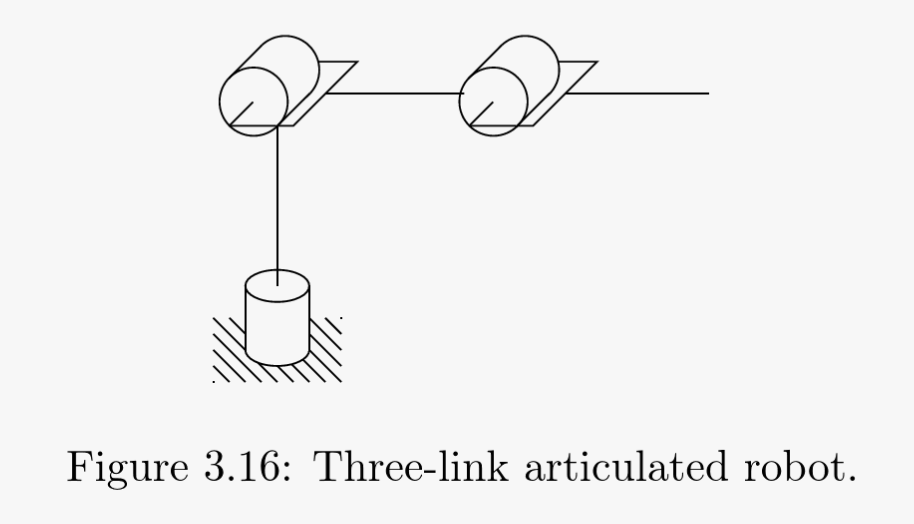
\includegraphics[scale=0.25]{figure3-16.png}
        \centering
    \end{figure}

    \textbf{Solution}
    \vspace{0.1in}\\
    First we assign coordinate frames 0 through 3 (links 0 through 3). This is done as per the following figure.
    \begin{figure}[h]
        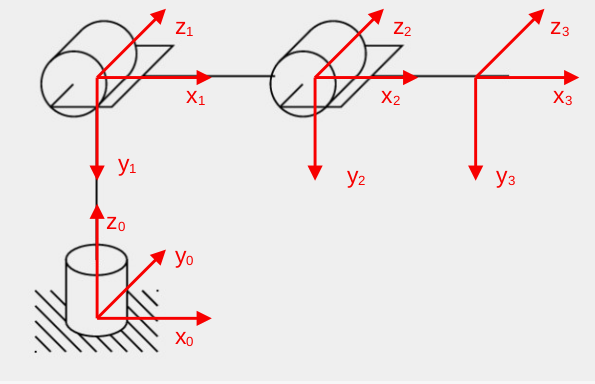
\includegraphics[scale=0.4]{problem-3-5-figure-frames.png}
        \centering
    \end{figure}

    Now, we create a table for quantities \(\alpha_i, a_i, \theta_i, d_i\) for links 1 through 3.

    \begin{table}[h!]
        \begin{center}
            \begin{tabular}{|c|c|c|c|c|}
            \hline
            Link & $\alpha_i$ & $a_i$ & $\theta_i$ & $d_i$ \\
            \hline
            1 & -90\degree & 0 & $\theta_1$ & $d_1$ \\
            2 & 0 & $a_2$ & $\theta_2$ & 0\\
            3 & 0 & $a_3$ & $\theta_3$ & 0\\
            \hline
            \end{tabular}
        \end{center}
    \end{table}

    Next, we use the matrix obtained from equation 3.10 of the textbook to calculate \(A_1, A_2, A_3\).
    
    \[
        A_1 =
        \begin{bmatrix}
            \cos\theta_1 & -\sin\theta_1\cos(-90\degree) & \sin\theta_1\sin(-90\degree) & 0\cdot\cos\theta_1\\
            \sin\theta_1 & \cos\theta_1\cos(-90\degree) & -\cos\theta_1\sin(-90\degree) & 0\cdot\sin\theta_1\\
            0 & \sin(-90\degree) & \cos(-90\degree) & d_1\\
            0 & 0 & 0 & 1
        \end{bmatrix}
        =
        \begin{bmatrix}
            c_1 & 0 & -s_1 & 0\\
            s_1 & 0 & c_1 & 0\\
            0 & -1 & 0 & d_1\\
            0 & 0 & 0 & 1
        \end{bmatrix}
    \]
    
    \vspace{0.2in}
    Where \(s_1 = \sin\theta_1\) and \(c_1 = \cos\theta_1\). Similarly,

    \[
        A_2 =
        \begin{bmatrix}
            c_2 & -s_2 & 0 & a_2c_2\\
            s_2 & c_2 & 0 & a_2s_2\\
            0 & 0 & 1 & 0\\
            0 & 0 & 0 & 1
        \end{bmatrix},
        A_3 =
        \begin{bmatrix}
            c_3 & -s_3 & 0 & a_3c_3\\
            s_3 & c_3 & 0 & a_3s_3\\
            0 & 0 & 1 & 0\\
            0 & 0 & 0 & 1
        \end{bmatrix}
    \]

    \vspace{0.2in}
    Now we can find \(T_3^0 = A_1A_2A_3\). We use the following MATLAB code to compute this.

    \lstinputlisting{./prob3_5.m}

    \vspace{0.2in}
    Therefore,
    \[
        T_3^0 =
        \begin{bmatrix}
            c_{1}\,c_{2}\,c_{3}-c_{1}\,s_{2}\,s_{3} & -c_{1}\,c_{2}\,s_{3}-c_{1}\,c_{3}\,s_{2} & -s_{1} & d_{1}+a_{2}\,c_{1}\,c_{2}-a_{3}\,c_{1}\,s_{2}\,s_{3}+a_{3}\,c_{1}\,c_{2}\,c_{3}\\
            c_{2}\,c_{3}\,s_{1}-s_{1}\,s_{2}\,s_{3} & -c_{2}\,s_{1}\,s_{3}-c_{3}\,s_{1}\,s_{2} & c_{1} & a_{2}\,c_{2}\,s_{1}-a_{3}\,s_{1}\,s_{2}\,s_{3}+a_{3}\,c_{2}\,c_{3}\,s_{1}\\
            -c_{2}\,s_{3}-c_{3}\,s_{2} & s_{2}\,s_{3}-c_{2}\,c_{3} & 0 & d_{1}-a_{2}\,s_{2}-a_{3}\,c_{2}\,s_{3}-a_{3}\,c_{3}\,s_{2}\\
            -c_{2}\,s_{3}-c_{3}\,s_{2} & s_{2}\,s_{3}-c_{2}\,c_{3} & 0 & d_{1}-a_{2}\,s_{2}-a_{3}\,c_{2}\,s_{3}-a_{3}\,c_{3}\,s_{2}\\
            0 & 0 & 0 & 1
        \end{bmatrix}
    \]
    
    \vspace{0.2in}
    This gives the configuration of frame 3 with respect to the base frame (frame 0).

\end{homeworkProblem}

\nobreak\extramarks{Problem 3.6}{}\nobreak{}

\pagebreak

\begin{homeworkProblem}[3.6]

    Consider the three-link Cartesian manipulator of Figure 3.17. Derive the forward kinematic equations using the DH convention.
    \begin{figure}[h]
        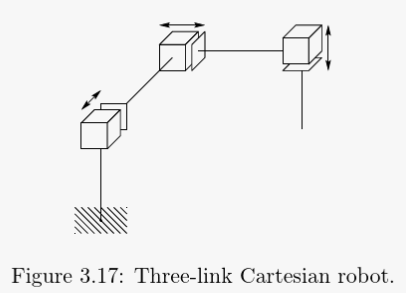
\includegraphics[scale=0.5]{figure-3.17.png}
        \centering
    \end{figure}

    \textbf{Solution}
    \vspace{0.1in}\\
    First we assign coordinate frames 0 through 3 (links 0 through 3). This is done as per the following figure.
    \begin{figure}[h]
        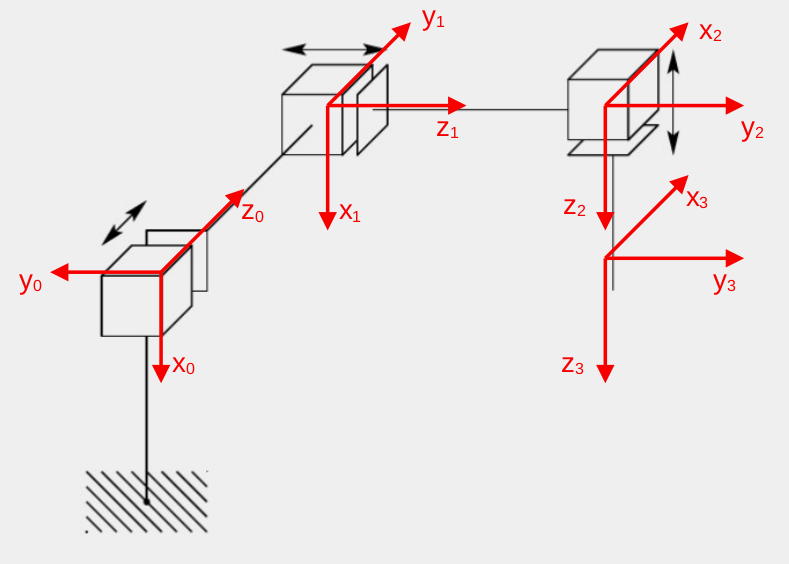
\includegraphics[scale=0.35]{figure3-17-frames.png}
        \centering
    \end{figure}

    \vspace{0.2in}

    Now, we create a table for quantities \(\alpha_i, a_i, \theta_i, d_i\) for links 1 through 3.

    \vspace{0.2in}

    \begin{table}[h!]
        \begin{center}
            \begin{tabular}{|c|c|c|c|c|}
            \hline
            Link & $\alpha_i$ & $a_i$ & $\theta_i$ & $d_i$ \\
            \hline
            1 & 90\degree & 0 & 0 & $d_1$ \\
            2 & 90\degree & 0 & 90\degree & $d_2$\\
            3 & 0 & 0 & 0 & $d_3$\\
            \hline
            \end{tabular}
        \end{center}
    \end{table}

    \vspace{0.1in}

    Next, we use the matrix obtained from equation 3.10 of the textbook to calculate \(A_1, A_2, A_3\).

    \[
        A_1 =
        \begin{bmatrix}
            1 & 0 & 0 & 0\\
            0 & 0 & -1 & 0\\
            0 & 1 & 0 & d_1\\
            0 & 0 & 0 & 1
        \end{bmatrix},
        A_2 =
        \begin{bmatrix}
            0 & 0 & 1 & 0\\
            1 & 0 & 0 & 0\\
            0 & 1 & 0 & d_2\\
            0 & 0 & 0 & 1
        \end{bmatrix},
        A_3 =
        \begin{bmatrix}
            1 & 0 & 0 & 0\\
            0 & 1 & 0 & 0\\
            0 & 0 & 1 & d_3\\
            0 & 0 & 0 & 1
        \end{bmatrix}
    \]

    \vspace{0.2in}
    Now we can find \(T_3^0 = A_1A_2A_3\). We use the following MATLAB code to compute this.

    \lstinputlisting{./prob3_6.m}

    \vspace{0.2in}
    Therefore,

    \[
        T_3^0 =
        \begin{bmatrix}
            0 & 0 & 1 & d_{3}\\
            0 & -1 & 0 & -d_{2}\\
            1 & 0 & 0 & d_{1}\\
            0 & 0 & 0 & 1
        \end{bmatrix}
    \]

    \vspace{0.2in}
    This gives the configuration of frame 3 with respect to the base frame (frame 0).
    
\end{homeworkProblem}

\nobreak\extramarks{Problem 5.3}{}\nobreak{}

\pagebreak

\begin{homeworkProblem}[5.3]

    Solve the inverse position kinematics for the cylindrical manipulator of Figure 5.15.
    \begin{figure}[h]
        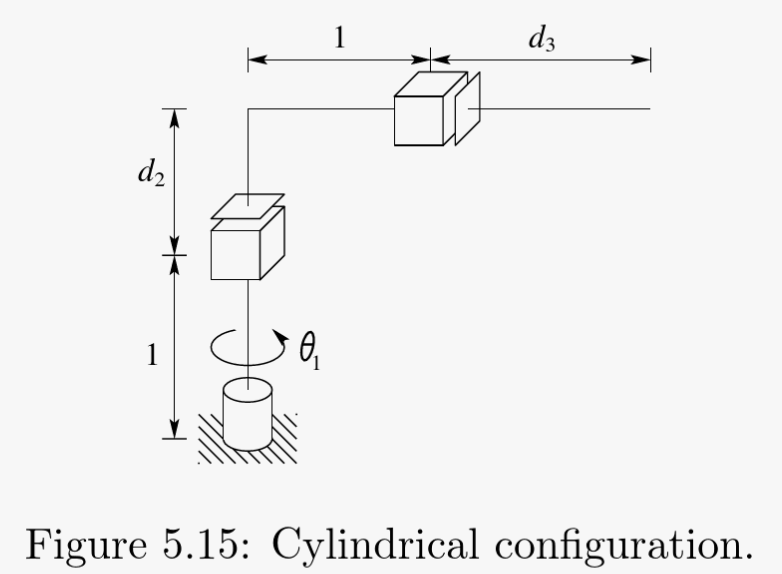
\includegraphics[scale=0.3]{figure-5.3.png}
        \centering
    \end{figure}

    \textbf{Solution}
    \vspace{0.1in}\\
    Let us draw the base frame's axes $x_0 y_0 z_0$ as shown in the figure below. Also, let us
    select a point $(x_c, y_c, z_c)$ as the wrist center at the far end of the second prismatic joint, as shown.
    \begin{figure}[h]
        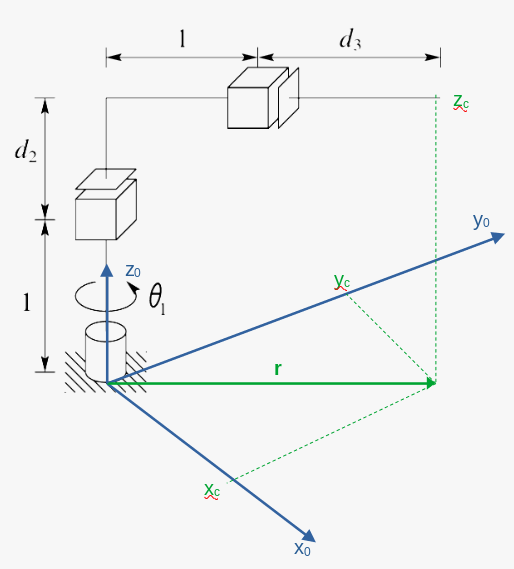
\includegraphics[scale=0.45]{figure-5.3-sketched.png}
        \centering
    \end{figure}

    \vspace{0.2in}
    To solve the inverse position kinematics problem for this configuration, we need to find $q_1, q_2, q_3$, or more precisely, $\theta_1, d_2, d_3$.

    \vspace{0.2in}
    Using the $Atan2()$ algorithmic function as described in the appendix of the textbook, we determine from the figure that,

    \[
        \boxed{\theta_1 = Atan2(x_c, y_c)}
    \]
        
    or, alternatively,
        
    \[
        \boxed{\theta_1 = \pi + Atan2(x_c, y_c)}
    \]

    \vspace{0.2in}
    Furthermore, it is apparent that

    \[
        \begin{split}
            z_c = 1 + d_2\\
            \boxed{d_2 = z_c - 1}
        \end{split}
    \]

    We also see from the figure that

    \[
        r = \sqrt[]{{x_c}^2 + {y_c}^2}
    \]

    But,

    \[
        r = 1 + d_3
    \]

    So,

    \[
        \boxed{d_3 = \sqrt[]{{x_c}^2 + {y_c}^2} - 1}
    \]

    \vspace{0.2in}
    This solves the inverse position kinematics problem for the given cylindrical configuration.

\end{homeworkProblem}

\nobreak\extramarks{Problem 5.5}{}\nobreak{}

\pagebreak

\begin{homeworkProblem}[5.5]
    Add a spherical wrist to the three-link cylindrical arm of Problem 5--3 and write the complete inverse kinematics solution.
    \vspace{0.2in}

    \textbf{Solution}
    \vspace{0.1in}\\
    Let us consider a spherical wrist identical to the one used in the textbook. We attach this spherical wrist such that the wrist center,
    now denoted by vector $o_c$, coincides with the point $(x_c,y_c,z_c)$ as we found in Problem 5--3. We have concluded that the wrist center
    lies at this point because axes \(z_3, z_4, z_5\) intersect at this point. This point is also where the origins \(o_3, o_4, o_5\) lie as 
    per the frame assignment by DH conventions. We also know that the position of $o_c$ does not change despite \(\theta_4, \theta_5, \theta_6\)
    being variables.\\
    
    Also, for the sake of clearly denoting $d_3$ as joint variable $q_3$, we have now used $u_3$ in the figure. It is still the same distance 
    found in Problem 5--3, i.e. \(u_3 = \sqrt[]{{x_c}^2 + {y_c}^2} - 1\). Given our placement of frame 2, we now have $d_3 = u_3 + 1$. Therefore,
    \(q_3 = d_3 = \sqrt[]{{x_c}^2 + {y_c}^2}\).\\

    An additional thing to note is that although $z_6$ is along the same direction as $z_5$, the coordinates of $o_6$ lie on the point shown by
    the vector $o_6$.
    \begin{figure}[h]
        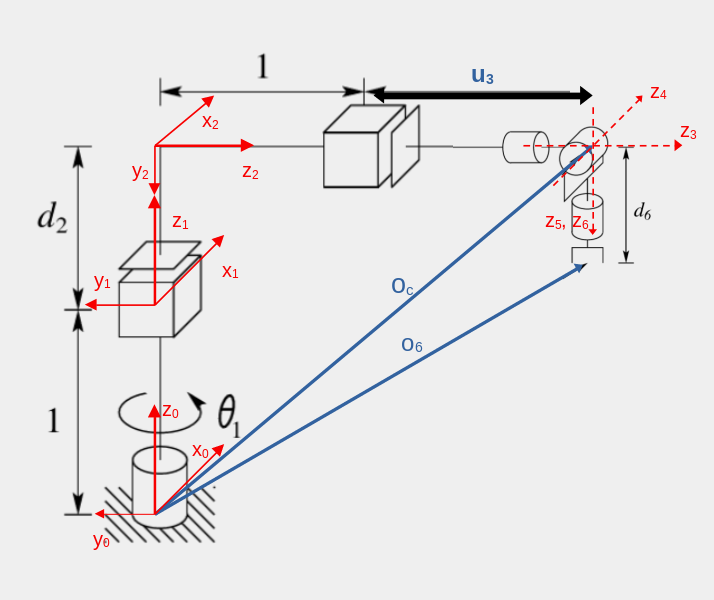
\includegraphics[scale=0.45]{figure-5.5-sketched.png}
        \centering
    \end{figure}

    Before we proceed further, let us make a brief list of steps we need to take to solve the complete inverse kinematics problem for our 
    particular manipulator's configuration.
    \begin{enumerate}
        \item Find wrist center $o_c$.
        \item Find $q1, q2, q3$.
        \item Perform forward kinematics to arrive at \(R^0_3 = {(R^3_0)}^T\).
        \item Get \(R^3_6 = R^3_0R^0_6\).
        \item Use $R^3_6$ to find $\phi, \theta, \psi$ of Euler configuration to find $q_4, q_5, q_6$.
    \end{enumerate}
    In essence, once we have found all joint variables given the end-effector's homogeneous transformation, we have solved the inverse kinematics problem.\\

    \textbf{Step 1}

    The end-effector's homogeneous transformation is known to us as the $4\times4$ matrix

    \[
        H^0_6 =
        \begin{bmatrix}
             R^0_6 & o^0_6\\
             0 & 1
        \end{bmatrix}
    \]

    where

    \[
        R^0_6 = 
        \begin{bmatrix}
            r_{11} & r_{12} & r_{13}\\
            r_{21} & r_{22} & r_{23}\\
            r_{31} & r_{32} & r_{33}
        \end{bmatrix},
        o^0_6 =
        \begin{bmatrix}
            x_6 \\
            y_6 \\
            z_6
        \end{bmatrix}
    \]

    Where $o^0_6$ is $o_6$ as shown in the diagram. As shown in the figure, we can establish a relationship between $o_6$ and $o_c$ as

    \[
        \begin{split}
            o_c = o_6 - d_6R^0_6
            \begin{bmatrix}
                0\\
                0\\
                1
            \end{bmatrix}\\
            \begin{bmatrix}
                x_c \\
                y_c \\
                z_c
            \end{bmatrix}
            =
            \begin{bmatrix}
                x_6 - d_6r_{13} \\
                y_6 - d_6r_{23} \\
                z_6 - d_6r_{33}
            \end{bmatrix}
        \end{split}
    \]

    

    Where $d_6$ is a scalar.
    \vspace{0.15in}

    \textbf{Step 2}
    
    We have already found $q_1, q_2, q_3$ in Problem 5.3. We summarize our findings here,

    \[
        q_1 = \theta_1 = Atan2(x_c, y_c)\\
    \]
    \[
        q_2 = d_2 = z_c - 1\\
    \]
    \[
        q_3 = d_3 = \sqrt[]{{x_c}^2 + {y_c}^2}
    \]

    We have discarded the second possibility of $q_1$ as our choice.

    \vspace{0.15in}

    \textbf{Step 3}

    We perform forward kinematics for the first three joint variables. Here is our table,

    \begin{table}[h!]
        \begin{center}
            \begin{tabular}{|c|c|c|c|c|}
            \hline
            Link & $\alpha_i$ & $a_i$ & $\theta_i$ & $d_i$ \\
            \hline
            1 & 0 & 0 & $\theta_1$ & 1 \\
            2 & 90\degree & 0 & 0 & $d_2$ \\
            3 & 0 & 0 & 0 & $d_3$\\
            \hline
            \end{tabular}
        \end{center}
    \end{table}
    
    Next, we use the matrix obtained from equation 3.10 of the textbook to calculate \(A_1, A_2, A_3\).

    \[
        A_1 =
        \begin{bmatrix}\cos\left(\theta _{1}\right) & -\sin\left(\theta _{1}\right) & 0 & 0\\ \sin\left(\theta _{1}\right) & \cos\left(\theta _{1}\right) & 0 & 0\\ 0 & 0 & 1 & 1\\ 0 & 0 & 0 & 1 \end{bmatrix}
        ,
        A_2 = \begin{bmatrix} 1 & 0 & 0 & 0\\ 0 & 0 & -1 & 0\\ 0 & 1 & 0 & d_{2}\\ 0 & 0 & 0 & 1 \end{bmatrix}
        ,
        A_3 = \begin{bmatrix} 1 & 0 & 0 & 0\\ 0 & 0 & -1 & 0\\ 0 & 1 & 0 & d_{2}\\ 0 & 0 & 0 & 1 \end{bmatrix}
    \]
\end{homeworkProblem}

\nobreak\extramarks{ROS2 Report}{}\nobreak{}

\pagebreak

\section{Report for ROS2 Portion}

\end{document}